\chapter{Background and inspiration}

\epigraph{It has to start somewhere \\ it has to start sometime \\ what better place than here? \\ what better time than now?}{Guerrilla Radio \\ Rage Against the Machine, 1999}

\section{Research at MIT}

As part of the research that directly inspired this thesis, here are some courses, projects, and studies I have undertaken while at MIT Media Lab.

\subsection{Classes at MIT}

\begin{enumerate}
  \item Fall 2019, CMS.901 Current Debates in Media, by professor Sasha Costanza-Chock
  \item Fall 2019, MAS.S65 Recreating The Past, by professor Zach Lieberman
  \item Spring 2020, MAS.826 Sound: Past and Future, by Tod Machover
  \item Spring 2020, MAS.712 Learning Creative Learning, by professor Mitchel Resnick
\end{enumerate}

In the class Current Debates in Media, topics covered included fake news, surveillance, algorithmic bias, data colonialism, climate justice, algorithms of oppression, among others. For my final paper I wrote on the role of the media during the 2019 Chilean protests.

In the class Recreating the Past, I learned about media arts history, and I furthered my learning of the language C++ which I ended up using for writing the library for my thesis, and of the package and community of openFrameworks, which is one of the most popular open source frameworks for media arts.

In the class Sound: Past and Future, I learned more about the history of different computational advancements for sound, with a strong focus on projects at MIT Media Lab's own research groups including Opera of the Future, Hyperinstruments, and Music, Mind, and Machine.

\subsection{Projects at MIT}

Some other projects I created during these years include:

\begin{enumerate}
  \item SiguesAhi: an instrument to detect when oppressive institutions have ceased to exist. It is achieved with microcontrollers with Internet connectivity.
  \item Open Drawing Machine, with Gaurav Patekar: an open source low cost programmable drawing machine
  \item Introduction to networks for artists: a series of tutorials for beginners, to learn how to set up their own networks and collaborate in peer-to-peer ways for making art.
\end{enumerate}

\begin{figure}[ht]
  \centering
  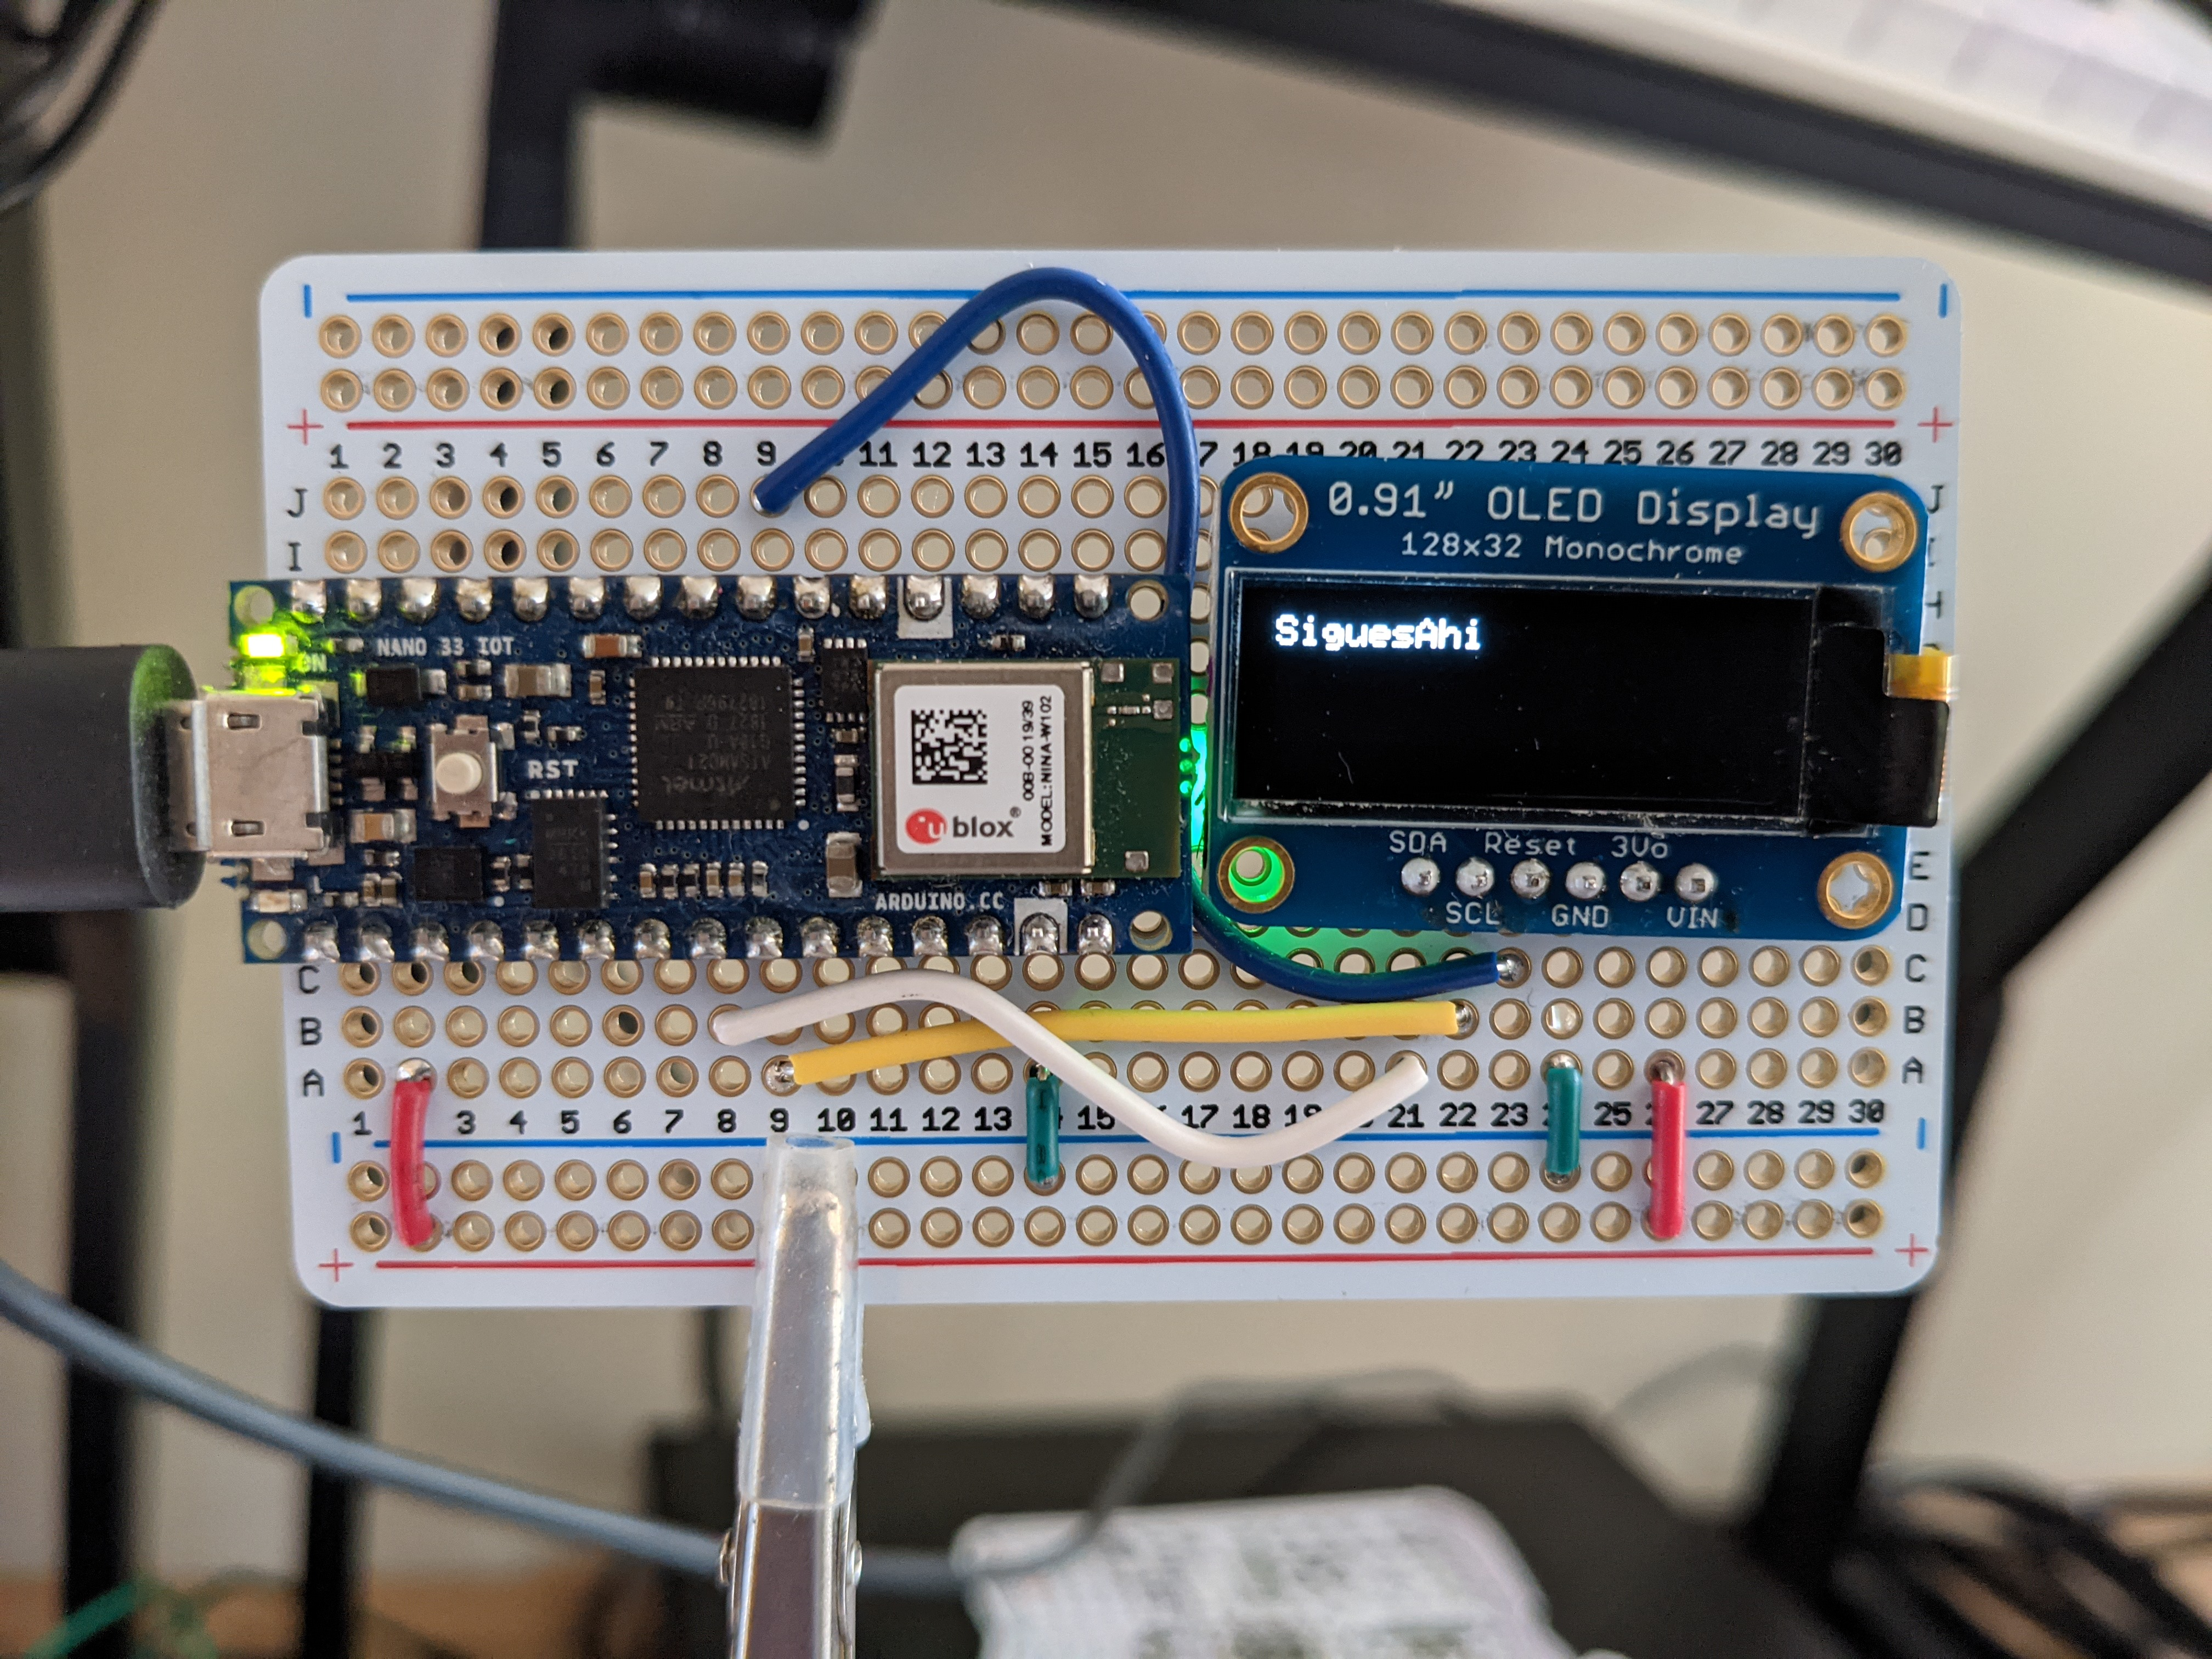
\includegraphics[width=0.75\linewidth,height=0.25\textheight,keepaspectratio]{images/sigues-ahi.jpg}
  \caption{SiguesAhi project}
  \caption*{Picture taken at home}
  \label{fig:sigues-ahi}
\end{figure}

\section{Computational media arts instruments}

On top of the proliferation of personal portable computers capable of performing real-time audio, and their creative live use by compute

In particular, here I will highlight some media arts instruments that have inspired my research, because of their use and promotion of open source software and hardware, scripting capabilities, and other design considerations. These instruments often sit at my desk for inspiration, or I spend hours playing with them for my art and learning from them and the communities around them.

The tables \ref{table:media-arts-instruments-technical} and \ref{table:media-arts-instruments-influence} are respectively a technical and influence summary of the instruments that I reference in this section.

\begin{table}[ht]
    \centering
    \begin{tabular}{ | l |  l | l | l | l |}
        \hline
        Company             & Instrument    & Year  & Computing & Software            \\
        \hline
        Bastl Instruments   & Kastle Drum   & 2020  & MCU       & Arduino, C++        \\
        Bastl Instruments   & Kastle v1.5   & 2017  & MCU       & Arduino, C++        \\
        Bastl Instruments   & microGranny 2 & 2016  & MCU       & Arduino, C++        \\
        Bastl Instruments   & Servo         & 2016  & MCU       & Arduino, C          \\
        Critter \& Guitari  & Organelle     & 2016  & Linux     & Pure Data           \\
        Critter \& Guitari  & EYESY         & 2020  & Linux     & Python, Pygame      \\
        monome              & aleph         & 2013  & Linux     & C                   \\
        monome              & norns         & 2018  & Linux     & Lua, SuperCollider  \\
        Shbobo              & Shnth         & 2013  & MCU       & Shlisp              \\
        Shbobo              & Shtar         & 2017  & MCU       & Shlisp              \\
        \hline
    \end{tabular}
    \caption{Technical details of media arts instruments}
    \label{table:media-arts-instruments-technical}
\end{table}{}

\begin{table}[ht]
    \centering
    \begin{tabular}{ | l |  l | l |}
        \hline
        Company             & Instrument    & Influence \\ 
        \hline
        Bastl Instruments   & Kastle v1.5   & placeholder \\
        Bastl Instruments   & microGranny 2 & placeholder \\
        Bastl Instruments   & Servo         & placeholder \\
        Critter \& Guitari  & Organelle     & placeholder \\
        Critter \& Guitari  & EYESY         & placeholder \\
        monome              & aleph         & placeholder \\
        monome              & norns         & placeholder \\
        Shbobo              & Shnth         & placeholder \\
        Shbobo              & Shtar         & placeholder \\
        \hline
    \end{tabular}
    \caption{Influence of media arts instruments}
    \label{table:media-arts-instruments-influence}
\end{table}{}

\subsection{Bastl Instruments}

Bastl Instruments is a Czech company of multimedia instruments, which has had a huge impact and influence on my research and practice. When I first started researching the Eurorack format some years ago, I visited the shop Control in Brooklyn NY, and some modules by Bastl stood out to me, because of their wooden panels and interaction with classic physical computing educational materials, such as motors and solenoids, which was an inspiration for me to include support for servo motors in Tiny Trainable Instruments.

\begin{figure}[ht]
  \centering
  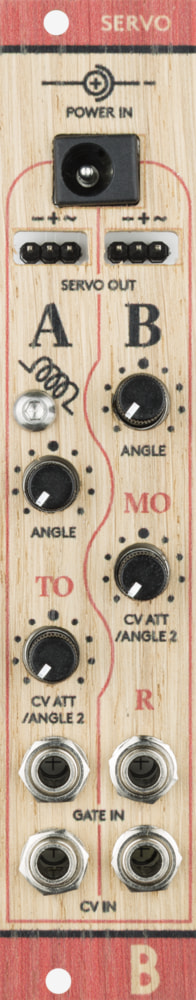
\includegraphics[width=0.75\linewidth,height=0.25\textheight,keepaspectratio]{images/bastl-servo.jpg}
  \caption{Bastl Instruments Servo module}
  \caption*{Retrieved from \cite{website-bastl-instruments-current}}
  \label{fig:bastl-servo}
\end{figure}

Another inspiration comes from their microgranny 2 granular sampler which is made with an Atmega microcontroller and its firmware is open source and available as a repository on their GitHub account, along with many other of their instruments.

\begin{figure}[ht]
  \centering
  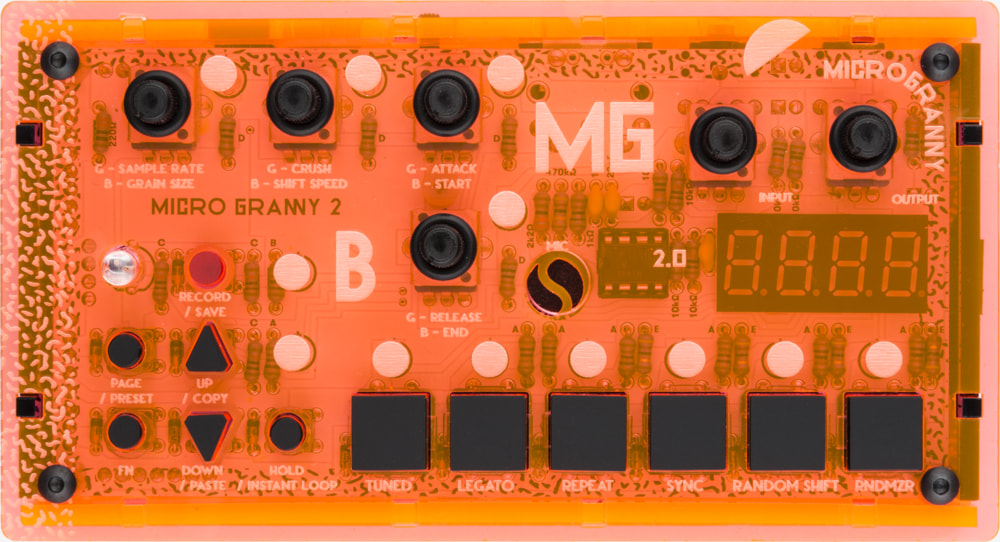
\includegraphics[width=0.75\linewidth,height=0.25\textheight,keepaspectratio]{images/bastl-microgranny-2.jpg}
  \caption{Bastl Instruments microGranny 2}
  \caption*{Retrieved from \cite{website-bastl-instruments-current}}
  \label{fig:bastl-microgranny-2}
\end{figure}

Their Kastle synthesizers are also based on microcontrollers, and feature a patchbay for making connections with jumper wires, the same used for prototyping in electronic breadboards, which influenced me to make the Tiny Trainable Instruments built with breadboards and jumper wires, instead of custom printed circuit boards. Also, the Kastle sythns are forgiving instruments, their inputs and outputs are robust enough to allow for mistakes in connections, in an electrical and mechanical way, which I think it's perfect for safe experimentation, it would be a bummer if the instrument was easy to break, or if it demanded a huge effort in understanding electronics for using it.

\begin{figure}[ht]
  \centering
  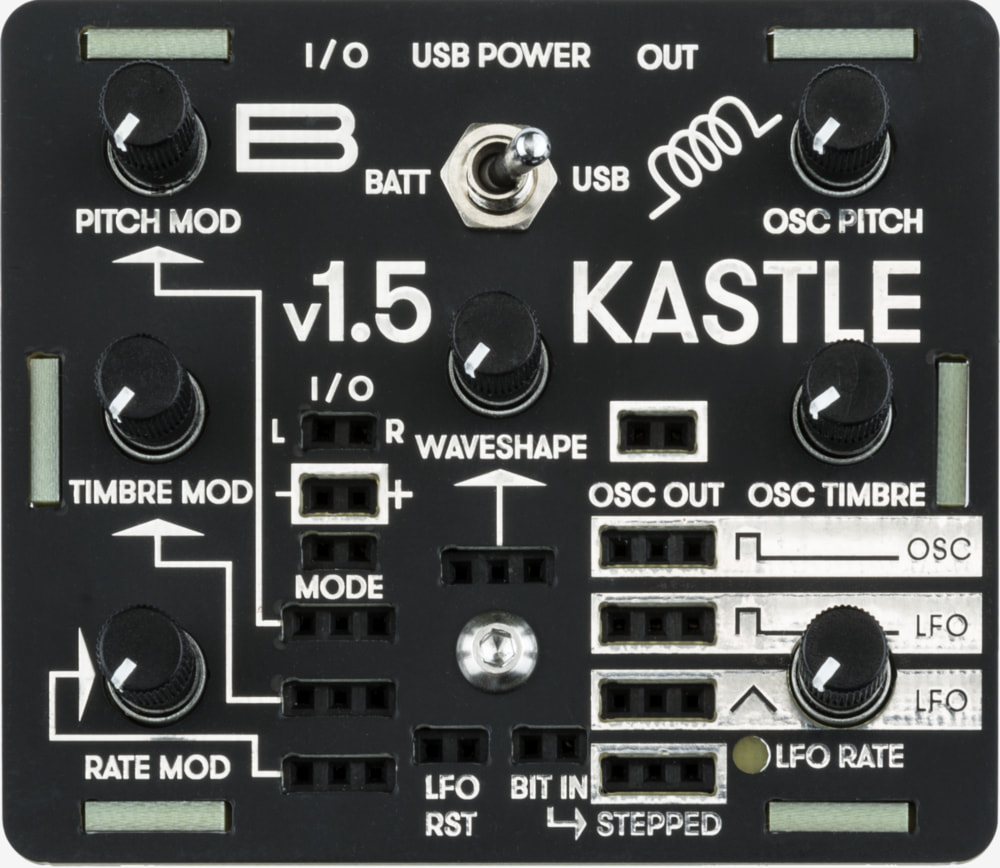
\includegraphics[width=0.75\linewidth,height=0.25\textheight,keepaspectratio]{images/bastl-kastle-v15.jpg}
  \caption{Bastl Instruments Kastle v1.5}
  \caption*{Retrieved from \cite{website-bastl-instruments-current}}
  \label{fig:bastl-kastle-v15}
\end{figure}

As of writing, 2 different units are in production, both retailing for ~100.00 USD, the Kastle v1.5 melodic / drone synthesizer, and the Kastle Drum, for rhythm. The only difference between these synthesizers is the firmware and the labels on the faceplate. The community is encouraged to write new firmware to modify their behavior. 

\begin{figure}[ht]
  \centering
  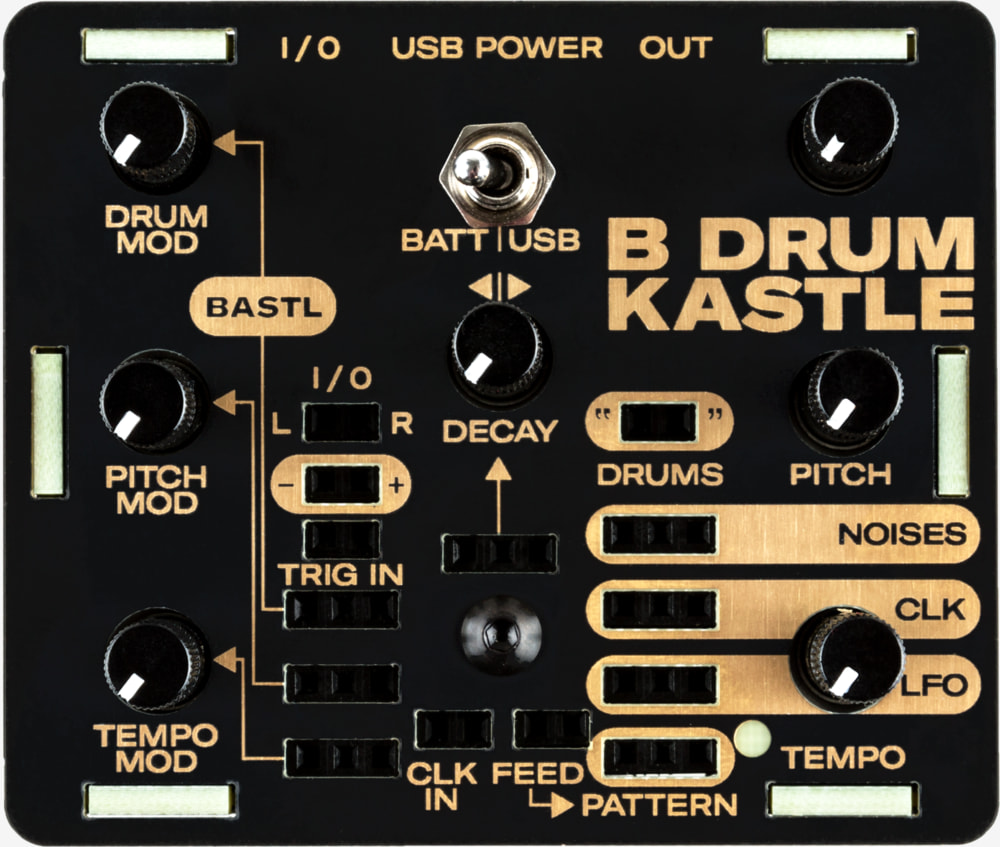
\includegraphics[width=0.75\linewidth,height=0.25\textheight,keepaspectratio]{images/bastl-kastle-drum.jpg}
  \caption{Bastl Instruments Kastle Drum}
  \caption*{Retrieved from \cite{website-bastl-instruments-current}}
  \label{fig:bastl-kastle-drum}
\end{figure}

Another instrument I want to highlight is the Illuminati, currently discontinued, a device that uses different inputs (audio, control voltage, MIDI messages), to control the light intensity of connected USB lamps, which influenced the conception of Tiny Trainable Instruments as multimedia arts instruments, not only focusing on audio and music, but also printed text, light, and screen output.

\begin{figure}[ht]
  \centering
  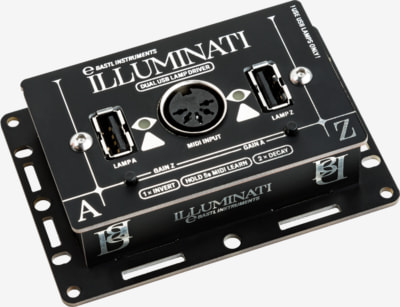
\includegraphics[width=0.75\linewidth,height=0.25\textheight,keepaspectratio]{images/bastl-illuminati.jpg}
  \caption{Bastl Instruments Illuminati}
  \caption*{Retrieved from \cite{website-bastl-instruments-current}}
  \label{fig:bastl-illuminati}
\end{figure}

The final instrument from this company that I want to highilight is the OMSynth, one of many collaborations with Casper Electronics. This device is an educational and maker circuit development tool for creating synthesizers, it includes basic fundamental blocks, such as battery power, audio input and output, potentiometers for attenuating and boosting signals, and a suite of parts kits for building devices including sequencers, oscillators, and samplers, on the included breadboard. Its release as a kit was also a direct influence in the release of Tiny Trainable Instruments as a kit with instructions.

\begin{figure}[ht]
  \centering
  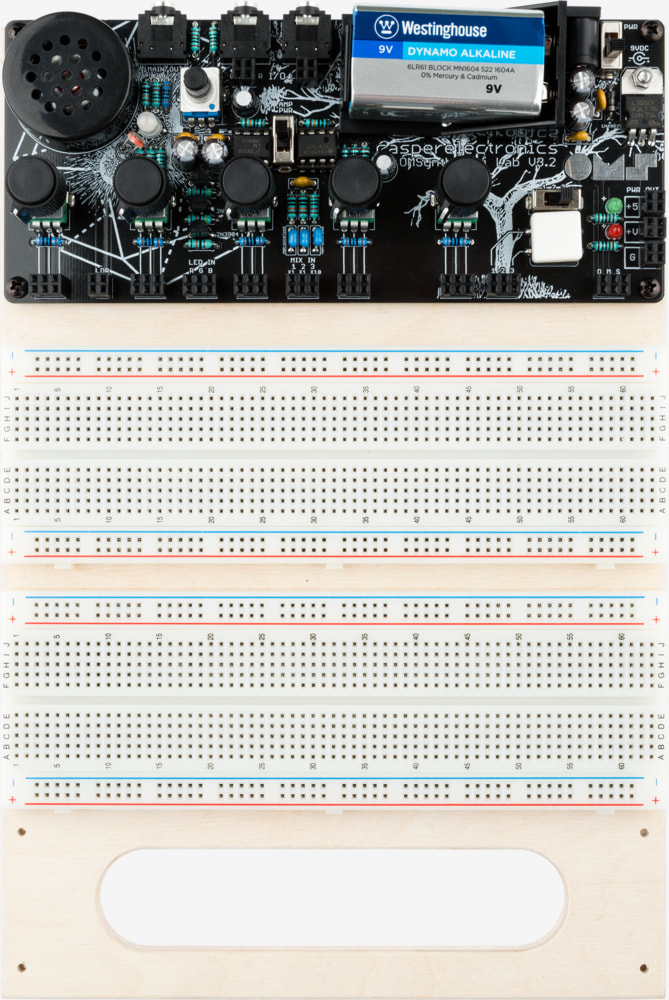
\includegraphics[width=0.75\linewidth,height=0.25\textheight,keepaspectratio]{images/bastl-omsynth.jpg}
  \caption{Bastl Instruments OMSynth}
  \caption*{Retrieved from \cite{website-bastl-instruments-current}}
  \label{fig:bastl-omsynth}
\end{figure}

Many BASTL standalone instruments are 200.00 USD or less, which is a huge contrast to the 1960s, when a Moog analog system II cost 6,200.00 USD, which was enough to buy a small house \cite{analog-days}. Also, many of their instruments are sold as kits for building and soldering them yourself, for the cheaper cost and the added educational aspect of having a hands-on experience.

\subsection{Critter \& Guitari}

Critter \& Guitari is an American company based in Brooklyn NY, which have released in the past computational microcontroller-based audiovisual instruments, from which my favorite is the Kaleidoloop, currently discontinued. It is a sampler with an internal mic and speaker, that allows you to record audio and then control its output with 2 knobs for volume and playback rate. It is designed to be portable for doing field recordings, and it was an influence on the design of the Tiny Trainable Instruments library, which allows the construction of standalone instruments, that with a USB power bank or a battery, you can take for a walk or place anywhere you want.

\begin{figure}[ht]
  \centering
  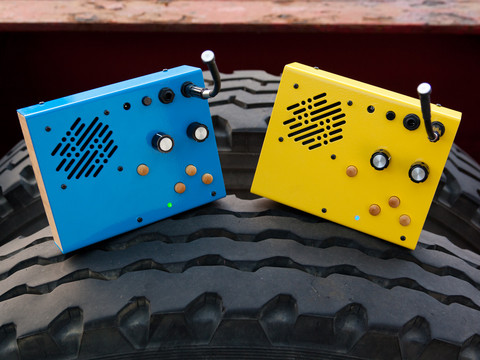
\includegraphics[width=0.75\linewidth,height=0.25\textheight,keepaspectratio]{images/critter-and-guitari-kaleidoloop.jpg}
  \caption{Critter \& Guitari Kaleidoloop}
  \caption*{Retrieved from \cite{website-critter-and-guitari-kaleidoloop}}
  \label{fig:critter-and-guitari-kaleidoloop}
\end{figure}

This company has released standalone scriptable computers for arts, which run Linux operating system + Pure Data software.

Organelle computer for sound, scriptable, Linux operating system + Pure Data software.

\begin{figure}[ht]
  \centering
  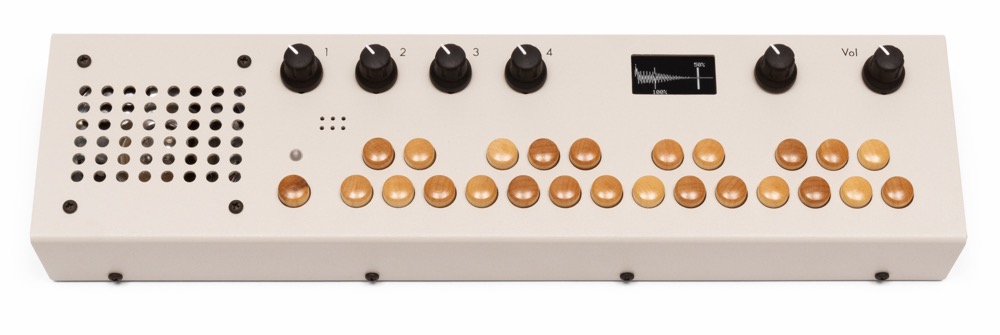
\includegraphics[width=0.75\linewidth,height=0.25\textheight,keepaspectratio]{images/critter-and-guitari-organelle-m.jpg}
  \caption{Critter \& Guitari Organelle M}
  \caption*{Retrieved from \cite{website-critter-and-guitari-current}}
  \label{fig:critter-and-guitari-organelle-m}
\end{figure}

ETC and EYESY computers for visuals, scriptable, Linux operating system + Python / pygame environment or openFrameworks.

\begin{figure}[ht]
  \centering
  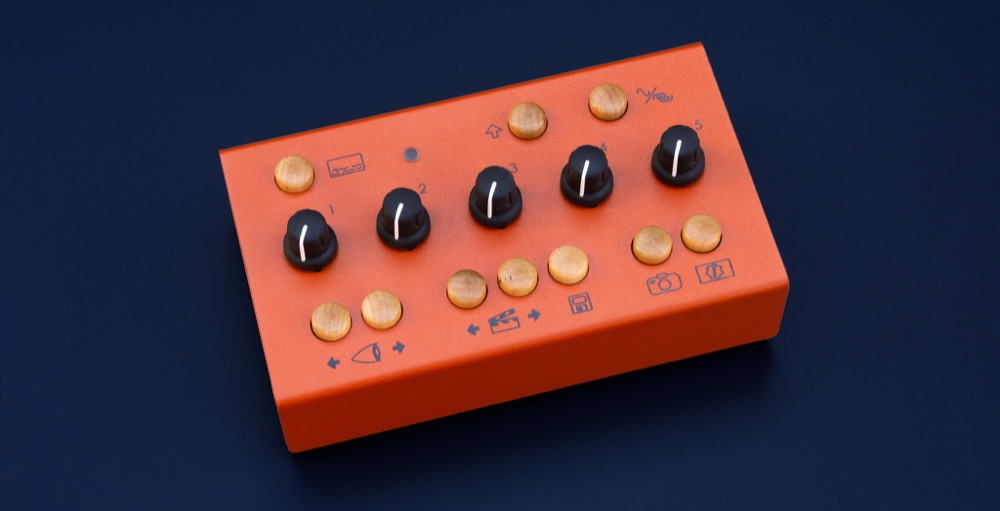
\includegraphics[width=0.75\linewidth,height=0.25\textheight,keepaspectratio]{images/critter-and-guitari-eyesy.jpg}
  \caption{Critter \& Guitari EYESY}
  \caption*{Retrieved from \cite{website-critter-and-guitari-current}}
  \label{fig:critter-and-guitari-eyesy}
\end{figure}

They can run on power supplies, and are also portable by the use of batteries.

\subsection{monome}

\begin{figure}[ht]
  \centering
  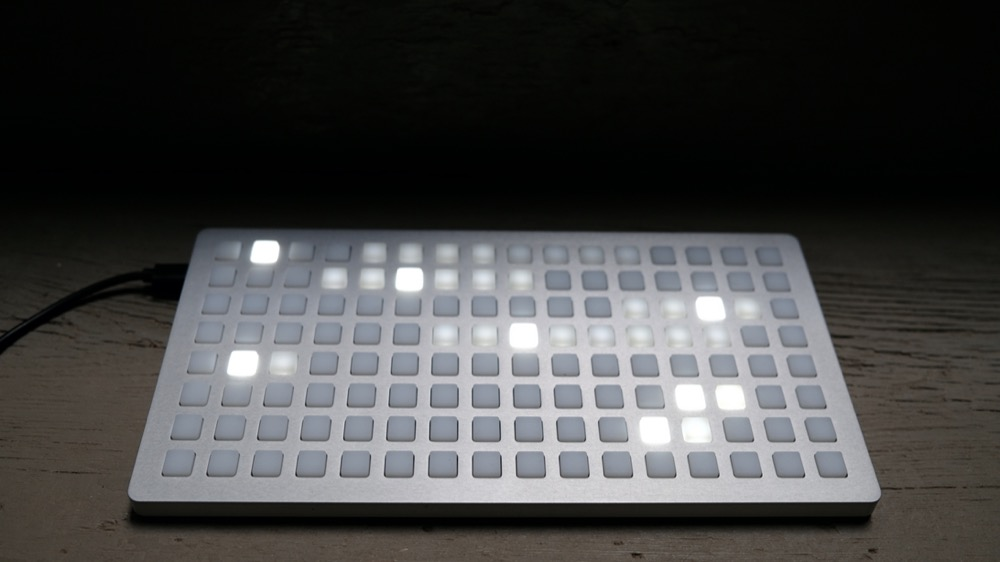
\includegraphics[width=0.75\linewidth,height=0.25\textheight,keepaspectratio]{images/monome-grid.jpg}
  \caption{monome grid}
  \caption*{Retrieved from \cite{website-monome-current}}
  \label{fig:monome-grid}
\end{figure}

Aleph: earlier sound computer.

Norns: sound computer, currently on its second iteration, with expanded hard drive. Also there is a DIY version which is cheaper and runs on a Raspberry Pi.
Norns is a Linux machine, running SuperCollider for the sound engine, and Lua scripts.

\begin{figure}[ht]
  \centering
  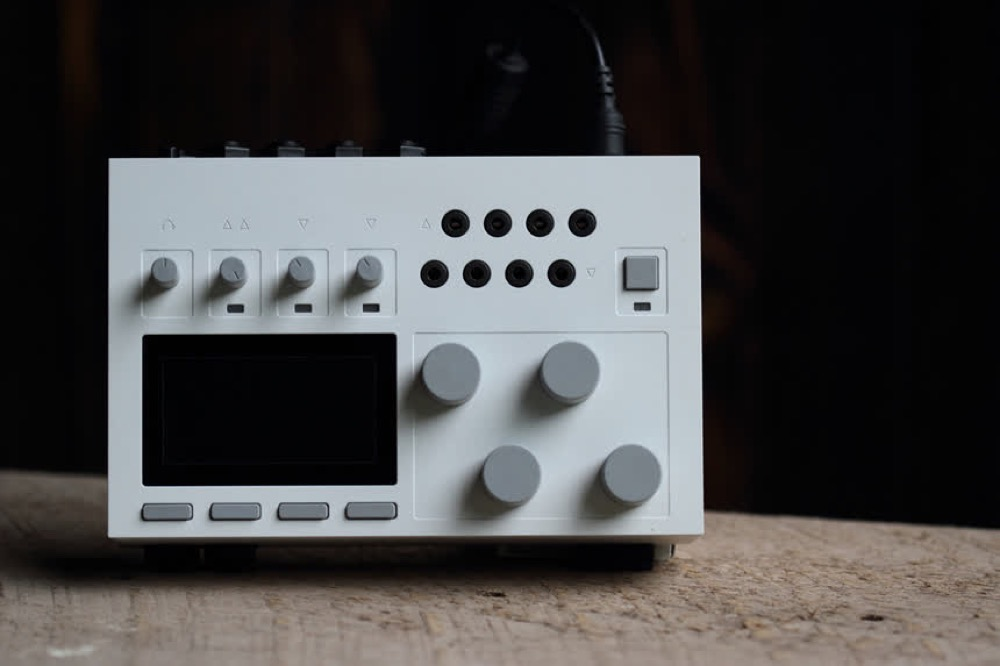
\includegraphics[width=0.75\linewidth,height=0.25\textheight,keepaspectratio]{images/monome-aleph.jpg}
  \caption{monome aleph}
  \caption*{Retrieved from \cite{website-monome-current}}
  \label{fig:monome-aleph}
\end{figure}

Norns: sound computer, currently on its second iteration, with expanded hard drive. Also there is a DIY version which is cheaper and runs on a Raspberry Pi.

Norns is a Linux machine, running SuperCollider for the sound engine, and Lua scripts. It has spawned a community that continually releases new scripts and software updates.

\begin{figure}[ht]
  \centering
  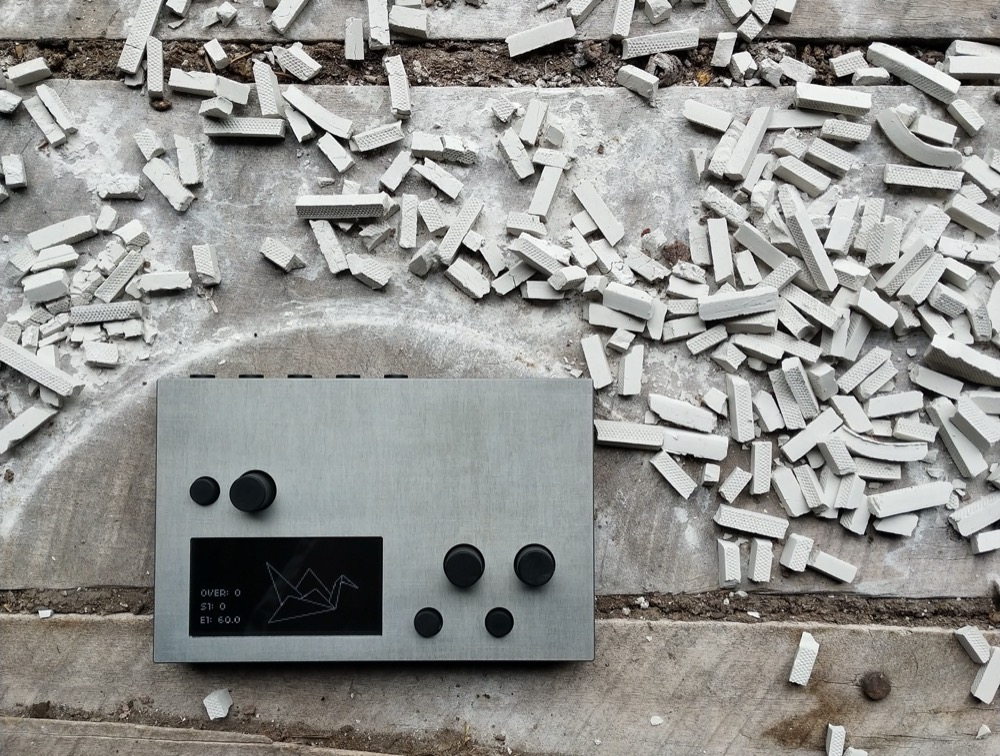
\includegraphics[width=0.75\linewidth,height=0.25\textheight,keepaspectratio]{images/monome-norns.jpg}
  \caption{monome norns}
  \caption*{Retrieved from \cite{website-monome-current}}
  \label{fig:monome-norns}
\end{figure}

\subsection{Shbobo}

Peter Blasser has released several collections / companies of musical instruments, the most famous one being Ciat-Lonbarde. Peter also runs Shbobo, which to date has two different instruments, the Shnth and the Shtar.

\begin{figure}[ht]
  \centering
  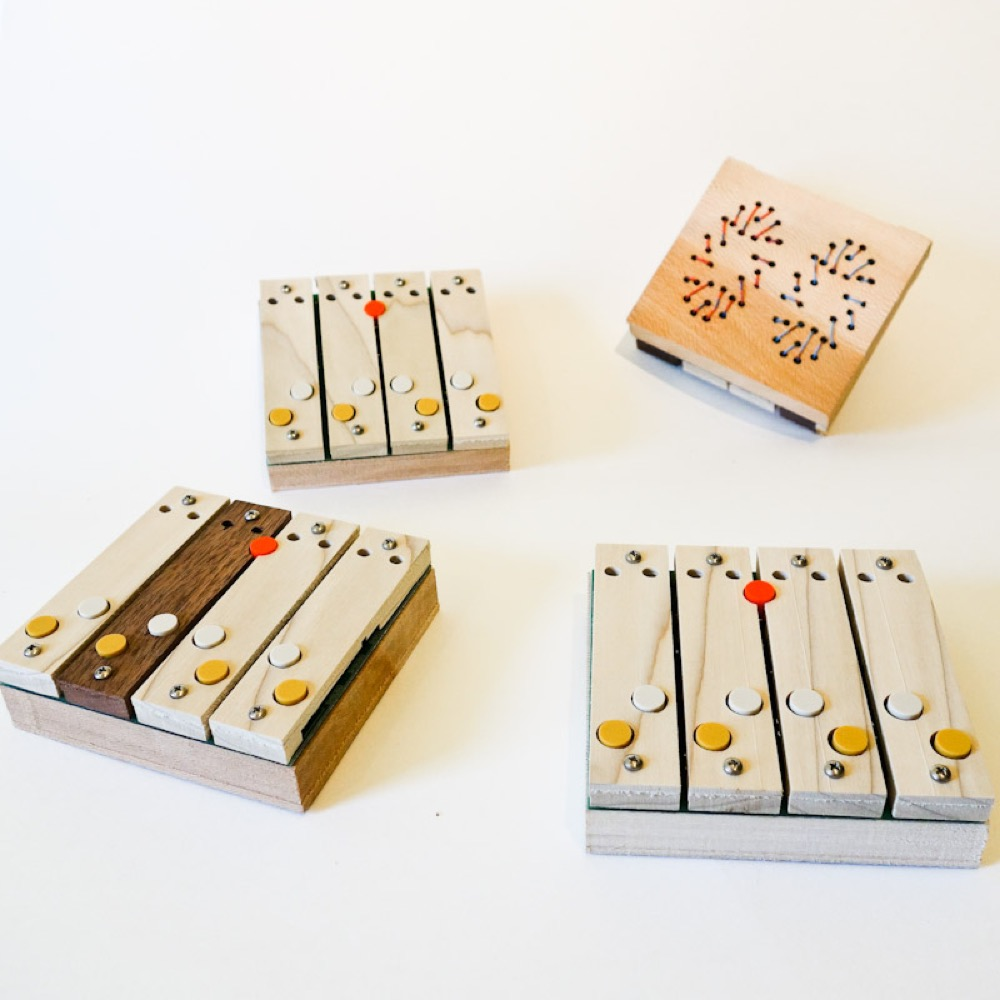
\includegraphics[width=0.75\linewidth,height=0.25\textheight,keepaspectratio]{images/shbobo-shnth.jpg}
  \caption{Shbobo Shnth}
  \caption*{Retrieved from \cite{website-shbobo-current}}
  \label{fig:shbobo-shnth}
\end{figure}

\begin{figure}[ht]
  \centering
    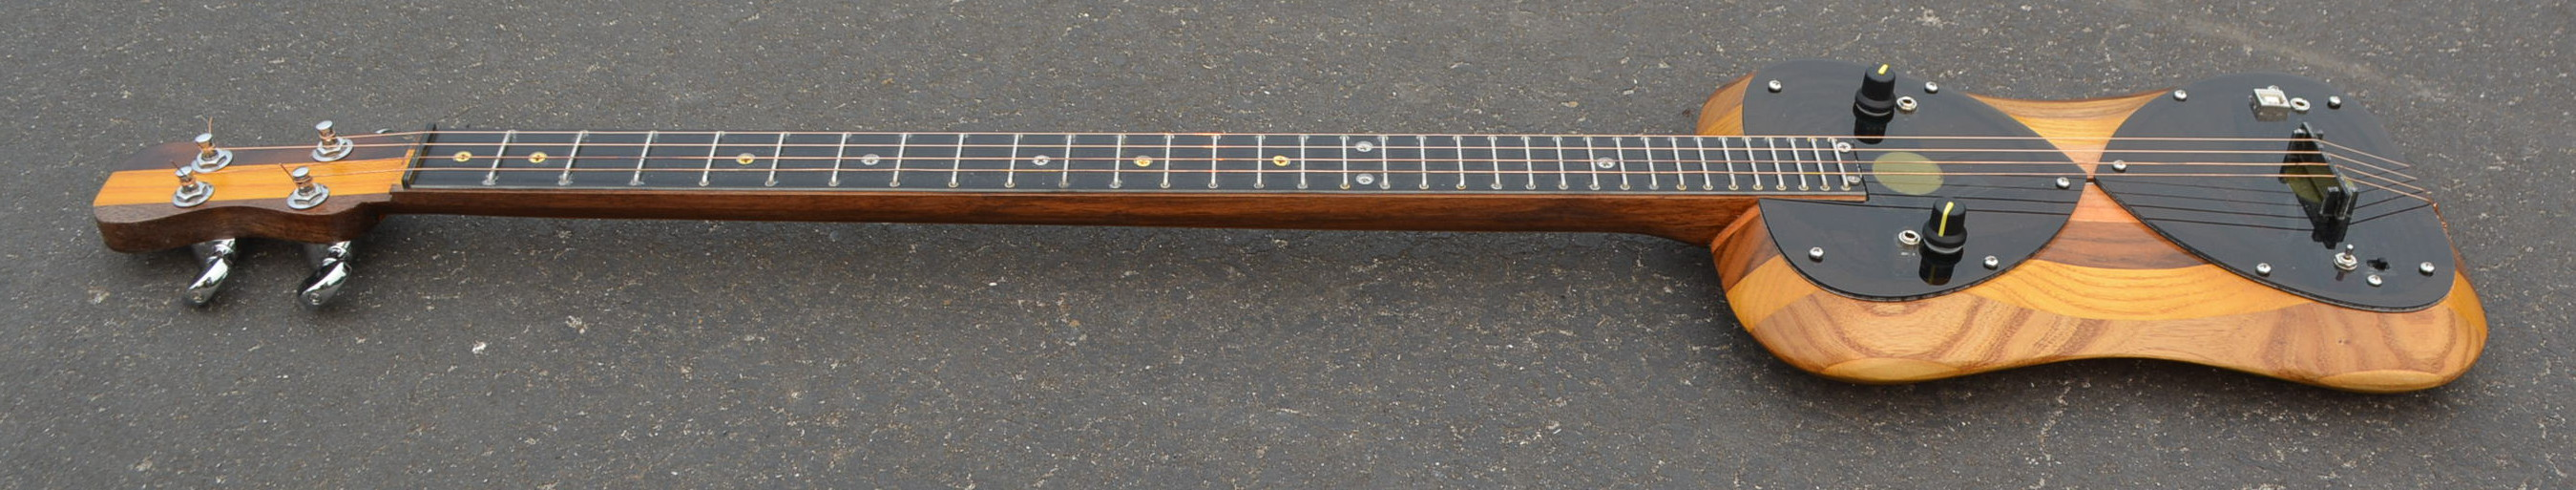
\includegraphics[width=0.75\linewidth,height=0.25\textheight,keepaspectratio]{images/shbobo-shtar.jpg}
  \caption{Shbobo Shtar}
  \caption*{Retrieved from \cite{website-shbobo-current}}
  \label{fig:shbobo-shtar}
\end{figure}

Both run on microcontrollers, and they use a new proposed language called Shlisp, based on Lisp, and also they can be programmed using the Fish IDE.

As of 2021, their firmware and editor became open source, and it is available at github.com/pblasser/shbobo.

COMMENT ON OPEN SOURCE: something being open source doesn't necessarily mean it is accessible to a wider audience. is one of the goals of your work to create instruments that are accessible to a wider audience?

They promote computer-centric approaches to making sound, such as the use of integers and metaphors of finite state machines, and also allow for different ways of playing and sensing, such as the use of antennas for detecting hand distance, a microphone for detecting speech and whistling, and wooden bars with piezos for detecting pressure.

TODO: write how this inspired the new interactions i am inventing or appropriating for Tiny Trainable Instruments, such as a drum machine you can talk to, Alexa spinoff.

\section{Education}

This thesis is inspired by the work of the research group Lifelong Kindergarten at MIT Media Lab, led by professor Mitchel Resnick. On the book with the same title, he builds on Seymour Papert’s work, and proposes that educational projects should have “Low floor, wide walls, high ceilings”, and that learners thrive when they engage in the 4 Ps: “Peers, projects, passion, play”.

In terms of peers, I have been lucky to have been supported by the MIT UROP office and MIT Media Lab, and had the opportunity to work with MIT undergrad researchers Peter Tone and Maxwell Wang. Also, this project was taught in collaborative workshops where people could discuss their ideas with their peers.

In terms of projects, this thesis includes the release of a software library, so that people can make the software their own, and spin-off their own projects. It is also open source so that people can learn from my mistakes and also fork to adapt to their needs.

In terms of passion, this thesis is 

In terms of play, this thesis project is not about correct answers, or even excellent classification with machine learning, it's all about finding innovative ways to interact with multimedia material, celebrate the small victories and the big glitches, and iterate over and over again.

\section{Creative machine learning}

COMMENT: what is the main argument of the whole piece and how does each independent part connect to that? you should start with a story from previous experiences that is particularly relevant as to why you were inspired to do this work. think "papert and the gears"

While being a graduate student and research resident at NYU ITP I saw how quick things changed in terms of machine learning. I saw how the project deeplearn.js allowed for people to train and deploy machine learning on their browsers, and how this library was acquired by Google and repurposed as TensorFlow.js, a JavaScript version of their machine learning framework TensorFlow.

In turn, at NYU ITP a team of artists and programmers built the library and community of ml5.js, with the 5 being an homage to p5.js. Technically, ml5.js is a wrapper for TensorFlow.js, in the same spirit that p5.js is a wrapper for HTML5 elements such as the canvas.

Another huge contribution to the landscape of machine learning for arts has been the release of the app Runway, which started as Cristóbal Valenzuela’s thesis, and is now a company with Alejandro Matamala and Anastasis Germanidis.

After leaving NYU ITP in 2018, I was a student at the month-long workshop “Autonomous Generative Spirit” taught by Gene Kogan and Andreas Refsgaard at the School of Machines, Make and Make Believe in Berlin 2018. We experimented with quick and cheap methods for machine learning, such as the k-nearest neighbors algorithm using the artist and beginner-friendly app Wekinator by Rebecca Fiebrink, and also more computer-intensive algorithms, which sometimes required proprietary hardware such as NVIDIA graphics cards to be trained in a matter of hours, instead of days or weeks using our computers.

There is a tradeoff between speed and cost, and also between monetary cost and time cost.

\begin{figure}[ht]
  \centering
    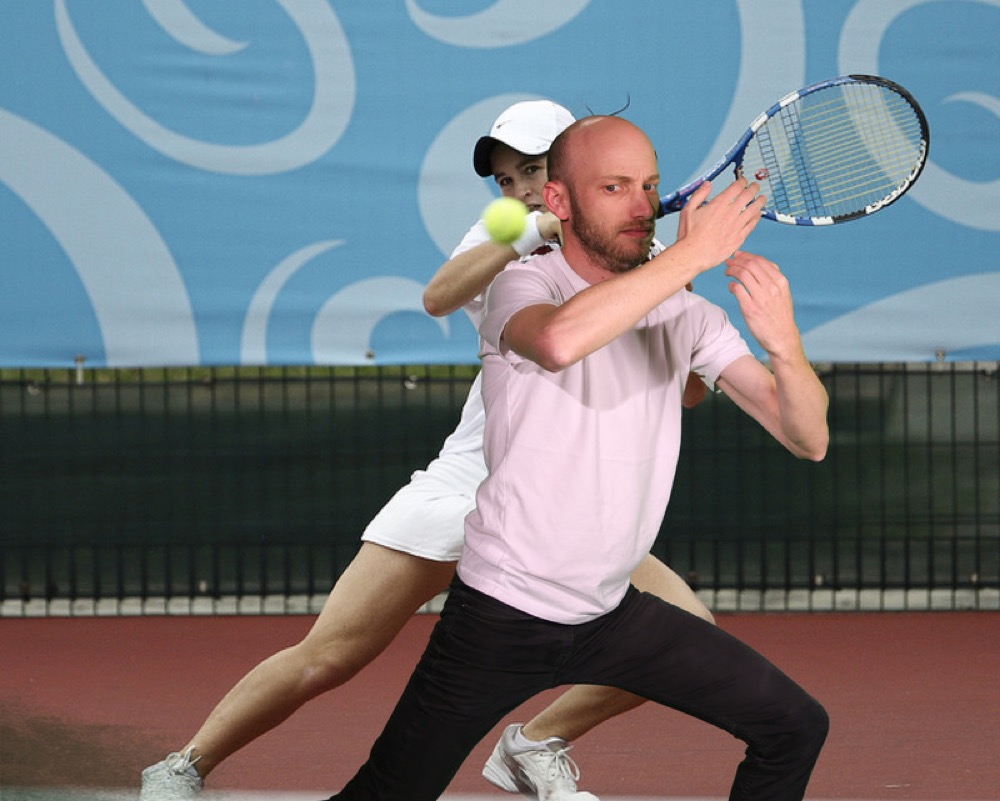
\includegraphics[width=0.75\linewidth,height=0.25\textheight,keepaspectratio]{images/sam-lavigne-training-poses.jpg}
  \caption{Sam Lavigne, Training Poses, 2018}
  \caption*{Retrieved from \cite{website-sam-lavigne-training-poses}}
  \label{fig:sam-lavigne-training-poses}
\end{figure}

The last spark that led me to this thesis was the release of 2 libraries for machine learning on the Arduino platform: The currently beta version Arduino KNN, which allows for on-device training and resembles my earlier studies with Wekinator, in a more portable and private way, no data leaves the microcontroller, and the whole neural network can be wiped with one click of a button.

At a more complex level, I am also working with the TensorFlow Lite Micro, which I learned from Arduino blogs, and which currently is supported by the hardware Arduino Nano 33 BLE Sense.

COMMENT TO THE ABOVE PARAGRAPH: you may not even need to include the specific details here, but just highlight in larger overviews the types of projects you've worked on or the educational fields that influence your work

In late 2020 and early 2021 I completed the just released series of 3 courses of the TinyML Professional Certificate by Harvard at the online platform edx.org

Newer books and references that this thesis was inspired by include the books “You Look Like a Thing and I Love You: How Artificial Intelligence Works and Why It's Making the World a Weirder Place” by Janelle Shane (2019), and the book “Making Pictures with Generative Adversarial Networks” by Casey Reas (2019).

Also Yining Shi created a new class at NYU ITP in 2020, at the intersection of machine learning and physical computing.

\section{Digital rights}

Machine learning algorithms need data to be trained on. I think it’s a human right to not be surveilled, and I hope my thesis can put a positive spin on the gathering of data, by letting users perform auto surveillance, like the Ai Weiwei piece WeiweiCam, a 2021 project where the artist installed cameras for self surveillance as a protest against the Chinese government.

A huge inspiration for my thesis has been the Guardian Project by the Electronic Frontier Foundation, and the research and activism work by Sasha Sasha Costanza-Chock.

\section{Education}

Mitch Resnick's book Lifelong Kindergarten

Low floor, wide walls, high ceiling

Peers, projects, passion, play

Gene Kogan and Andreas Refsgaard

\section{Machine learning}

ml5.js

Runway

TinyML Professional Certificate HarvardX

\section{Digital rights}

Electronic Frontier Foundation

Edward Snowden

Design Justice Network
